\section{Аналитическая часть}

\subsection{Постановка задачи}
	Необходимо разработать метод, который по заданной информации об элементах транспортной системы формировал бы рекомендации по объёмам и маршрутам поставки.

\subsection{Актуальность проблемы}
	В данный момент торговые розничные сети (другое название - ретейл) динамически развиваются и с каждым годом занимают всё большую долю в общем объёме розничной торговли\cite{subj:demand}. Деятельность подобных предприятий тесно связана с управлением цепочками поставок (SCM - Supply Chain Management) - комплекс подходов, помогающий эффективной интеграции поставщиков, производителей, дистрибьюторов
	и продавцов. Этот процесс можно разделить на следующие этапы\cite{subj:scm}. 
	\begin{enumerate}
		\item \textbf{Планирование}. Принимается решение об управлении жизненным циклом товаров, объёмах производства и закупок.
		\item \textbf{Закупки}. Происходит управление снабжением, оцениваются и выбираются поставщики.
		\item \textbf{Производство}. Включает в себя процесс производства, контроль технологических изменений, управление качеством и т.д.
		\item \textbf{Доставка}. Состоит из трёх основных процессов: управление заказами, управление складом и транспортировка.
		\item \textbf{Возврат}. На этом этапе определяются элементы возврата товара, составляются графики возврата и направления на уничтожение и переработку.
	\end{enumerate}
	
	Среди данных задач хочется выделить отдельно транспортную логистику. Затраты на неё являются существенными, что обосновывается её сложностью и жизненной важностью для деятельности фирмы. 
	
	Таким образом, расширение сегмента розничных сетей на рынке влечёт за собой повышение спроса на перевозку товаров. Большинство транспортных компаний прибегают к использованию программного обеспечения для ускорения и упрощения различных этапов процесса перевозки\cite{subj:auto_eff}.  Автоматизация данной работы позволяет повысить её эффективность и надёжность.

\subsection{Анализ предметной области}
	Целью деятельности транспортной логистики является организация перемещения груза между двумя местами по оптимальному маршруту\cite{subj:main}. В данном случае оптимальным считается тот маршрут, который позволяет перевезти объекты в предусмотренные сроки (желательно, минимальные) с наименьшими затратами и вредом для них. Стоит отметить, что зачастую возможные маршруты не являются оптимальными сразу по всем критериям, поэтому приходится принимать компромиссные решения.
	
	Случаи, когда задачи розничной торговли, транспортировки и складирования товара (а иногда даже производства) выполняются одной фирмой достаточно редки и характерны только для крупного бизнеса. Этот подход организации позволяет улучшить интеграцию всех перечисленных элементов логистической системы, что способно снизить издержки на каждом из этапов. Малые предприятия не располагают подобными ресурсами и, как правило, пользуются услугами других компаний для данной функции.  
	
	В рамках данной работы рассматривается решение задач автоматического планирования для автомобильной транспортной компании.
	
	Логистика малого бизнеса имеет ряд особенностей\cite{subj:small_business}. Как было отмечено, небольшие организации не способны содержать необходимый штат сотрудников, транспортных средств и т.д., а также не обладают достаточно большим оборотом товаров для собственной организации перевозки. Малые объёмы поставок для каждого отдельного предприятия приводят к тому, что компании-перевозчики совмещают планируют один маршрут сразу через несколько точек доставки.
	
	Можно заключить, что обыкновенный процесс работы фирмы доставки заключается в следующем. Несколько ретейл предприятий формируют заказы с указанием заказываемых товаров и их объёмов. Транспортная компания определяет совместные маршруты и средства доставки, формирует заказ для складского предприятия/ий. Назначенные грузовые автомобили загружаются на складе и развозят груз по нужным пунктам.

\subsection{Сравнение с аналогами}
	Системы управления перевозками (TMS - Transportation management system), как было отмечено выше, являются востребованными для предприятий, занимающихся логистикой. Данные системы, в основном, решают следующий перечень задач\cite{subj:tms_cmp}:
	\begin{itemize}
		\item расчет логистических затрат;
		\item оптимальное использование транспортных средств для минимизации
		общих расходов;
		\item повышение качества обслуживания - соблюдение сроков доставки, установленных транспортной службой компании;
		\item автоматизация процесса транспортного планирования и управления,
		обеспечивающая решение для конкурентного транспортного планирования
		и управления;
		\item повышение производительности труда работников при планировании и
		организации грузовых перевозок.
	\end{itemize}

	В число наиболее популярных в России входят следующие TMS.
	\begin{itemize}
		\item Oracle Transportation Management;
		\item 1С: TMS Логистика. Управление перевозками;
		\item SAP TM.
	\end{itemize}

	Перечисленные программы позволяют осуществлять составление, расчёт стоимостей, поручение и контроль выполнения транспортировок. Также зачастую реализуются различные интерфейсы и функционал для водителей, логистов и т.д. Таким образом, общей чертой данных систем является комплексный подход к решению задач транспортной логистики. Предпринимается попытка удовлетворить все потребности, так или иначе связанные с обработкой данных.   
	
	Однако среди указанных программ автоматическое планирование с учётом наиболее важных факторов позволяет Oracle TM. В случае других TMS планирование не реализовано настолько детально. Ввиду крайне высокой цены\cite{subj:tms_cmp} на Oracle Transportation Management и в целом на подобные программы, небольшие транспортные фирмы не могут позволить себе столь высокие расходы. Решением может быть использование представленной в этой работе программой в интеграции с сравнительно недорогой TMS, решающей другие задачи транспортного управления.
	

\subsection{Постановка задачи}
	Требуется разработать алгоритм, выполняющий планировку маршрутов доставки заказов от складов до потребителей (ретейл фирм). Целью создания продукта является определение таких маршрутов и транспортных средств, которые будут наиболее выгодными для компании. В первую очередь под выгодой подразумевается денежная прибыль.
	
	Целевой пользователь - логист транспортной компании. Для него применение программы нужно для получения рекомендаций по заданию маршрутов в определённый момент времени. После этого работник может проанализировать полученные маршруты, внести в них свои корректировки и заняться последующими этапами своей деятельности (непосредственно организации грузоперевозок, документооборотом и т.д.).
	
	Исходными данными является информация о следующих объектах:
	\begin{itemize}
		\item грузовые машины, входящие в автопарк фирмы;
		\item перевозимые товары;
		\item стоянка грузовиков;
		\item поставщики и потребители товара (в данном случае склады и розничные торговые фирмы);
		\item пути между вышеописанными пунктами маршрута;
		\item заказы.
	\end{itemize}

	Результатом работы должны стать предлагаемые маршруты. Схематически пример модели представлен на рисунке \ref{pic:model}, где стрелками обозначены маршруты, выбранные алгоритмом как оптимальные.
	
	\begin{figure}[h!] 
		\begin{center}
			{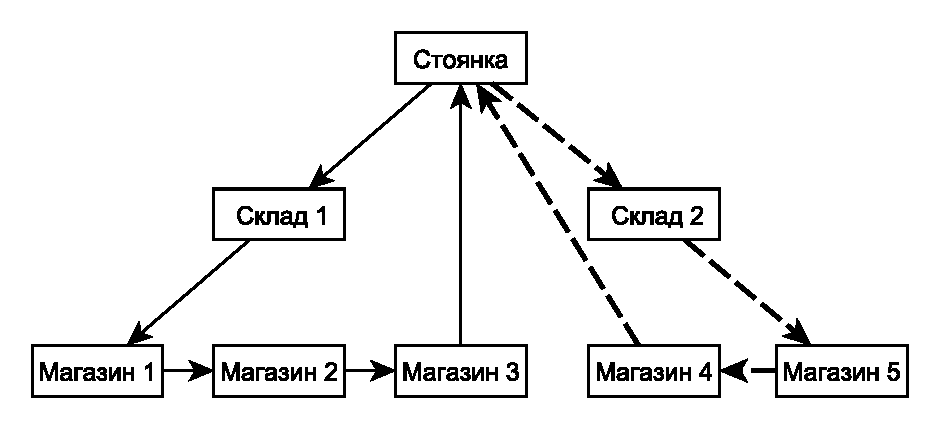
\includegraphics[scale=0.9, angle=0]{img/model.pdf}}
			\caption{Схема модели}
			\label{pic:model}
		\end{center}
	\end{figure}
	
	Рассмотрим упомянутые объекты, обозначим допущения и ограничения для задачи.
	
	Одним из главных вопросов является выделение критерия оптимизации, служащего для оценки решений. Как было отмечено выше, главным является денежная прибыль, то есть повышение доходов и уменьшение затрат.   
	Первый путь достигается только через выполнение наибольшего количества заказов. Однако, это может быть принято как данное -- будем считать, что выполнение всех заказов является обязательным. Это обусловленно большими штрафами, как правило существенно превышающими рассмотренные далее затратами.   
	Деятельность фирмы грузодоставки связана с множеством статей затрат, но пути перевозки влияют только на время и пробег грузовиков, что в свою очередь отражается на средствах, затрачиваемых на топливо. Для упрощения, будем считать, что этот расход можно вычислить используя длину маршрута и среднюю затрату на километр. Оценка по времени является так как одинаковое время затраченное в пробке и на свободной дороге ведёт к совершенно разным результатам.
	
	Путь между пунктами доставки достаточно описать с использованием только расстояния. Информация о времени проезда данного участка в момент планирования может стать неактуальной к проезду транспорта по нему. Поэтому данная информация не задаётся для путей. В случае временной непроходимости участка дороги информация о нём может быть заменена на альтернативный или вовсе удалена.
	
	Решение проблемы расположения разнородного груза в автомобиле и расчёта его вместимости в общем случае является достаточно сложной задачей. Так, например, хрупкие вещи могут не допускать расположение другого груза поверх них. Поставка товаров является оптовой в поставленной задаче, поэтому примем распространённый в этой сфере подход: все виды товаров поставляются в внутри тар, которые имеют определённый объём и не имеют специальных условий транспортировки. В таком случае также можно считать, что грузовик вмещает некоторые тары, если их суммарный объём не превышает заполняемый объём кузова.
	
	Первый и последний пункт любого рейса является автостоянка транспортной фирмы, причём в обоих случаях машина не содержит каких-либо грузов. Также будем считать, что посещение складов и потребителей не может происходить "вперемешку"\ - в первую очередь посещается склад, после чего товары из него доставляются в один или несколько пунктов. Это условие нужно для избежания длинных рейсов с промежуточными пополнениями.

\subsection{Формализация задачи}
	Сформулированная задача является задачей поиска оптимального решения, а именно транспортной задачей \cite{trans:main}. Она решает проблему составления плана перевозок из пунктов отправления в пункты потребления, который будет иметь наименьшие затраты на перевозки. 
	
	В простейшем случае модель транспортной системы рассматривается как множество пунктов производства однородного продукта и множество его потребителей. Известны затраты перевозки одной единицы товара для любой пары производителя и потребителя.
	
	Использование такой модели некорректно, так как она не учитывает следующие факторы.
	\begin{itemize}
		\item Склады и транспортные средства ограничены и обладают конечной вместимостью.
		\item Рассматриваемый магазин оперирует сразу множеством товаров. Это порождает сразу ряд дополнительных обстоятельств. Например, тары имеют различные габариты, что влияет на вместимость транспортного средства.
		\item Рассматриваются только маршруты "Производитель - Потребитель"\, тогда как в рассмотренной модели маршрут может проходить сразу через несколько потребителей. Таким образом и перевозимый одним транспортом груз зависит сразу от нескольких потребителей.
	\end{itemize}
		
	Основным способом решения вопроса множества продуктов сводится к условному разбиению поставщиков и потребителей из общих на работающих только с одним продуктом. Таким образом задача сводится к однопродуктовой с общим для всех разбиений одного пункта ограничением на пропускную способность.
	
	В таком случае рассмотрим математическую модель транспортной задачи для одного продукта.
	\paragraph{Формализация данных}
	Формализуем данные метода. В первую очередь обозначим основные величины: $Vol$ - объём одной тары, $Con$ - стоимость топлива (литр / у.е.)
	
	$A_i$ - склады с запасом продукции в $a_i$, ($i = \overline{1, N_a}$).
	
	$B_i$ - потребители с потребностью продукции в $a_i$, ($i = \overline{1, N_b}$).
	
	Данные об $A$ и $B$ и автостоянке можно объединить в понятие пункта маршрута $P$, где $a_i$ - количество продукта (в случае потребителя отрицательно, по модулю равно потребности, в случае стоянки - всегда 0), где $i = 1$ - автостоянка $i = \overline{2, N_a + 1}$ - склады, $i = \overline{N_a+2, N_b+N_a+1}$ - потребители. Общее количество пунктов опишем как $N = N_b+N_a+1$.
	
	$O_{(k-1) + i}$ - заказ $k$-м, сделанный потребителем $i$-м на $ov_{(k-1) + i}$ товаров (в тарах) к сроку $ot_{(k-1) + i}$, где $i = \overline{1, N_b}$, $k \ge 1$.
		
	$T_i$ - транспорт с вместимостью в $c_i$ (в кубометрах) и затратой топлива в $f_i$ (в литр / км) ($i = \overline{1, N_t}$). 
	
	Рейсы транспорта обозначим как $R_{(k-1)N_t + i}$, где $i = \overline{1, N_t}$ - номер транспорта $T_i$, $k \ge 1$ - номер рейса (в рассматриваемый период).
	
	Тогда $t_{ij} > 0, d_{ij} > 0$ - время перемещения и расстояние между $P_i$ и $P_j$, $v_{ijk} \ge 0$ - количество товара перевезённое $k$-м рейсом между $P_i$ и $P_j$, $i \ne j, i, j = \overline{1, N_b+N_a}$, $k = \overline{1, N_t}$. Вектор $v$, удовлетворяющий ниже идущим условиям и ограничениям считается \textbf{решением}.
	
	\paragraph{Формулирование условия решения}    
	План перевозок можно считать решением задачи в случае, если поставки удовлетворили всех потребителей. В принятом обобщении пунктов это можно записать как
	\begin{equation}
		a_i + \sum_{j=1}^{N_b+N_a} \sum_{k=1}^{N_t} (v_{jik} - v_{ijk}) \ge 0
	\end{equation}
	
	\paragraph{Формулирование ограничений}     
	
	Ни на одном из этапов перевозки объём продукта не должен превысить максимальную вместимость транспорта.
	\begin{equation}
		v_{ijk} \cdot Vol \le c_k, \forall i, j \in \overline{1, N_b+N_a}, k \in \overline{1, N_t}
	\end{equation}

	Обратные перевозки невозможны
	\begin{equation}
		v_{ijk} > 0 => v_{jik} = 0
	\end{equation}

	Транспорт может въехать и выехать из пункта только одним путём
	\begin{equation}
		\left\lbrace 
		\begin{array}{cols}
			\nexists i, k, j_1, j_2: j_1 \ne j_2, v_{ij_1k} > 0, v_{ij_2k} > 0 \\
			\nexists j, k, i_1, i_2: i_1 \ne i_2, v_{i_1jk} > 0, v_{i_2jk} > 0 
		\end{array}
	\end{equation}

	Все заказы должны быть выполненны в срок.	
	
	\paragraph{Формулирование критериев}   
	Критерием оптимизации является минимизация затрат. Как было отмечено выше, планирование способно оказывать влияние только на стоимости всех рейсов. Целевая функция принимает следующий вид.
	\begin{equation}
		L(v) = Con \cdot \sum_{i=1}^{N_b+N_a} \sum_{j=1}^{N_b+N_a} d_{ij} \cdot \sum_{k=1}^{N_t} v_{ijk} \to min
	\end{equation}

	\paragraph{Математическая модель}
	Приведём все описанные формализации в математическую модель рассматриваемой задачи поиска оптимального плана поставок.
	
	\begin{equation}
	\begin{array}{cols}		
		L(v) \to min \\
		\left\lbrace 
		\begin{array}{cols}
			a_i + \sum_{j=1}^{N_b+N_a} \sum_{k=1}^{N_t} (v_{jik} - v_{ijk}) \ge 0 \\
			\\
			v_{ijk} \cdot Vol \le c_k, \forall i, j \in \overline{1, N_b+N_a}, $k \in \overline{1, N_t}$ \\
			v_{ijk} > 0 => v_{jik} = 0 \\
			\nexists i, k, j_1, j_2: j_1 \ne j_2, v_{ij_1k} > 0, v_{ij_2k} > 0 \\
			\nexists j, k, i_1, i_2: i_1 \ne i_2, v_{i_1jk} > 0, v_{i_2jk} > 0 
		\end{array}
	\end{array}
	\end{equation}

\subsection{Метод решения}
	Учитывая перечисленные факторы, в качестве основы для решения сформулированной задачи возможно выбрать метод потенциалов в сетевой постановке. Он является модификацией симплекс-метода, применяющегося для многих оптимизационных задач, в том числе и классической транспортной задачи\cite{trans:potential}.
		
	Преимуществом такого метода является то, что он позволяет создавать транзитные маршруты через пункты потребления и добавлять ограничения на пропускную способность, что необходимо в данном случае. Для этого можно условно представить каждого потребителя складом на время отгрузки транспорта в нём. Вместимость такого склада равна неиспользованному месту в грузовике.
	
	Поддержка доставки множества видов продуктов можно добиться доработкой данного метода\cite{trans:polyprod}.
	
	...

\subsection*{Вывод}
	Результатом аналитического раздела стала постановка задачи, освещение актуальности проблемы. Была разработана математическая модель исследуемой системы, определён и описан метод решения.
\pagebreak